\chapter{Awful}

\section{A Constructed Image}

\keywords{superficial impressions, bitterness, false expectations}

\noindent -- Hello, how are you feeling today?\\
-- Awful.

This is not what a meditator is supposed to say, is it? They should
respond positively like, `I'm feeling great, it's such a lovely day!' Or
at least `I'm OK, and how are you?' We have an image of a `meditator' in
our heads who is supposed to behave and speak in certain ways, while not
behaving and speaking in certain other ways. Who has put that image in
\emph{my} head?

The image of the `good meditator' is a perception formed from
superficial impressions which, without deeper examination, we have
allowed ourselves to see as real. Imagine opening an article about
meditation (while continuing to read the current one\ldots). It starts
with the smiling photo of a monk or a lay meditation teacher, and it
continues by describing the positive effects of mindfulness. It might
include stories and photos taken at a retreat. People are sitting on
meditation cushions with serene faces while the light through the window
is illuminating the Buddha statue. The article might contain interview
excerpts about how participants had overcome their inner struggles. It
ends with the encouraging words of a meditation teacher, or with a quote
from the Buddha.

Even someone not terribly interested in meditation knows what this
article looks like, we have seen dozens of them. There is no need to
include a reference source, the chapters in this book could be examples
as well.

This is not to suggest they are being deceitful. The authors are acting
with good intentions. They are trying to encourage us to continue on the
path of contemplation and to put effort into our practice. If we can't
see a greater happiness beyond the frustrations, what would be the
point? If there was only suffering and misery to expect, we don't need
help in creating that.

\keywords{happiness, removing blocks from a river, vipassana-glamour}

Buddhism is fundamentally optimistic, and one of its central theme is
happiness. Our own attitude is that we seek happiness, or want to create
it. While we are occupied with that, however, we can become more and
more bitter, as it can seem that such happiness can never be realized.
We assume the fault is in our circumstances or personal abilities, and
we tend to reject what is already here, assuming that it can't be right.

This way of thinking is like trying to carve a statue which will be
\emph{just right}, but we are never satisfied with the result. We think
it's our fault, and we don't notice that the materials of the statue are
just the way they are. Clay will be clay, sand will be sand, stone will
be stone. The \emph{khandhas}, form, feeling, perception, mental
conditions, consciousness will be as they are. What creates the struggle
is when we expect them to be otherwise.

Effort is necessary, but a better metaphor could be that of a choked up
river: blocks of stone are in the way, creating turbulence and blocking
the flow of the water. The mind is inherently bright and
luminous\footnote{\href{https://suttacentral.net/an1.41-50/en/thanissaro}{AN
  1.49}, Luminous}, but when it is blocked up with sensual craving,
desire for various states of existence and obscured by ignorance (the
three \emph{āsavas}), it becomes dark and murky.

The teachings do mention suffering frequently, but such instruction is
given on the ground that freedom from that suffering is possible. The
Buddha made it clear that the fruit of the path is genuine happiness,
and if it was not possible to practise it, i.e. to abandon unwholesome
roots and develop the wholesome ones, he would not have taught
it.\footnote{\href{https://suttacentral.net/an2.11-20/en/thanissaro}{AN
  2.19}, Skillful}

Who is that meditator in our head? One thing is sure, the one in
\emph{my head} is always a \emph{better meditator} than I am. When
someone takes a good photo of us, we know how it is: it was a good
moment when we looked orderly or even glamorous, but we know that in
five minutes the opposite could be true. And although this is true not
just for us, somehow we don't remember this about good photos taken of
other people. These are a sort of \emph{vipassana}-glamour shots -- it's
a bit vain but we like looking at them. They make good illustrations in
an article, but we should remember that the same people will look
different in an ordinary moment.

\clearpage

\section{Threads}

\keywords{suttas as literature}

In the days of the Buddha, one form of literature was the \emph{sutta},
which means a thread of discourse. \emph{Suttas} may include prose
and/or verse, and were intended to be memorized through recitation. A
community would compose a \emph{sutta} after a significant event, such
as a discussion or formal a teaching, to give the story a formal
presentation in which they would memorize it. The Buddha certainly
encouraged them to do so:

\begin{quote}
Thus you should train yourselves: `We will listen when discourses that
are words of the Tathāgata---deep, deep in their meaning, transcendent,
connected with emptiness---are being recited. We will lend ear, will set
our hearts on knowing them, will regard these teachings as worth
grasping \& mastering.'

\bigskip

\quoteRef{%

\href{https://www.dhammatalks.org/suttas/SN/SN20_7.html}{SN 20.7}, The
Peg

}
\end{quote}

Today, books, articles and blog posts fulfil this function. These modern
media, in essence and at their best, hold up the canonical \emph{suttas}
as their example. The monks of the early years delivered their message
to us through these threads, and their efforts have become part of our
conversation with those we meet today, just as our written works will
speak to those in the future who we will never meet.

\keywords{social media, selection bias, Instagram Effect}

However, in today's social media the clear understanding of the message
is distorted by what is called `the Instagram effect', which is a
selection bias to show our best and most positive side, and filter out
the negative one, which is nonetheless just as real and necessary for
complete understanding.

This influence is not negligible, medical journals have already started
discussing a form of depression and obsessive behaviour called `Snapchat
Dysmorphia',\footnote{\href{https://www.ncbi.nlm.nih.gov/pmc/articles/PMC5933578/}{Is
  ``Snapchat Dysmorphia'' a Real Issue? (ncbi.nlm.nih.gov)}} in which
case the patient seeks cosmetic surgery to look more like the photos
they see in the application.

The automatic filters edit every picture to be more attractive, and if
we repeatedly see our bodies shown to us (by the application) as a
nearly flawless image, \emph{that} becomes our mental self-image, and
the unfiltered image we see in the mirror seems wrong to us.

One might consider a similar Instagram Effect in published articles
about meditation experiences. The author has a point to explain, and
they select a mix of personal experiences, opinions, and supporting
explanations from other authors.

The author may write truthfully and try to avoid selection bias, but
subtle, unconscious forms of self-filtering keep operating. They select
and present a slice of their own experience, building on examples
(hopefully) familiar to their readers. The world of the written text is
always a constructed reality. Nonetheless, when it works well, we
recognize our own experience in it, made clear by well-chosen words.

\clearpage

\keywords{mental images as role models}

The meditator who lives in our head is like a character in a poem, or
the hero in a myth. They can be wiser and stronger than we are, so that
when we are feeling lost and weak, they can give us faith and advice.
They can have unshakeable peace, so that when we are feeling awful, we
are able to endure and wait until the difficulty ends.

Such mental images are, however, just that, and shouldn't be mistaken
for a real person. They are valuable sources for guiding ourselves, the
narrative description helps us to figure out what to do by showing where
we are in a bigger picture. The role of a mental image is not what we
\emph{should become}. When we relate to perceptions and ideals like
that, we are going to feel conflicted and inadequate, because the real
circumstances of our life are far more complex, rich with ambiguous,
shifting boundaries and are not like the simplified reality of a mental
image. Mental images are tools for explanation. They are \emph{ways of
seeing} the world, and are examples of acting correctly in that kind of
world.

\clearpage

\section{Assumptions}

\keywords{mind and the world, mode of attention, actions and beliefs}

We may remember the verse in the Dhammapada which points out that the
world of our experiences is not independent of us:

\begin{quote}
Mind precedes all states of being: they are led by the mind, made by the
mind.

\bigskip

\quoteRef{%

\href{https://suttacentral.net/dhp1-20/pli/ms}{Dhp 1}

}
\end{quote}

How can we test whether we are creating imaginary problems for
ourselves, or if the pressure to act is an important sign which we
shouldn't ignore?

First, we may ask, `Can the subject experience suffering?' Living beings
can suffer, but a cultural idea or self-made story cannot suffer, even
while \emph{we are}. It changes our attitude if the subject of our
concern only exists as a story and not as a living being. Such
insentient stories include the narratives we have around institutions,
nations, money, fame, or other social fabrications.

A quick moral safety test may follow: `Would a wise person praise or
criticize doing this?'

Next comes remembering and untangling the view: `What assumption creates
this stress and pressure? What is the motivation for doing this? Without
what, would this have no significance?'

We can reveal such unconscious motivations by looking at our present
actions and choices. What we choose to do now expresses what we believe
in, the assumptions we have accepted in the past.

`Why am I choosing to do this, here? Where does this action come from
and where does it lead?'

The underlying factors for our actions may come, for example, from the
habitual conditioning of our environment. We may have not expressed in
thought why we do what we do, but have felt the results being
\emph{expressed on us}, whether good or bad.

Starting the investigation with a closer look at our actions and
\emph{then} asking about the thoughts motivating them can turn out to be
a more reliable method. This is because our inner chit-chat says all
sorts of contradictory things, but our actions give a clearer point of
reference.

\keywords{the best place to learn, reversing assumptions}

The associated feeling might be awful, but if we treat it as sign to
turn toward the mind and investigate it, our approach can stay practical
and productive. `If I am here anyway, what can I learn from this?'

We find access to our assumptions through uncovering our unconscious
motivations -- once we can express an assumption clearly, we gain the
freedom to reverse it, or drop it. We may ask, `Does it help in this
situation, if I reverse my assumptions?' Perhaps looking at it in the
opposite way is exactly what is we needed either for peace of mind, for
the clarity to continue, or for dropping the issue as if it never
existed. Either way, we are not acting out of compulsion: we are free to
either let it go or \emph{choose} to follow it through.

\clearpage

\section{After the Storm}

\keywords{happiness and accomplishments}

When instruction says, `return to the present moment', it doesn't mean
you must like everything you find there, but this is the only place
where you can live. If you are happy, you are not happy in the future,
but in the present. If you are suffering, you can't understand it in the
future, only in the present. In some situations, no amount of brainy
self-talk is going to make it better, it is best to call it the way it
is, and endure it with dignity. A conflict is genuinely stressful,
separation from what we love is going to be sad, and being alive always
ends with the tragedy of our own death.

We tend to anticipate success, and expect our hard work to be justified
in the future. Carefully examine that moment of accomplishment, what do
you experience? There may be surprise, joy, exhilaration, relief, and
then everything is back to the ordinary level. The destination turns out
to be not what we thought, and if we were intensely focused to get
there, we might not even remember anything from the journey, and regret
missing it. We can be so intent on being productive, that we waste our
chance to live.

\keywords{values, being busy, Hedonic Treadmill, contentment}

Contemplating death puts a truthful, if somewhat scary, mirror to our
values. `If I die tonight, would I be happy to remember living as I am
living today?' This question can stir up more from the deep recesses of
the psyche than we wish for. I remember a time when my response the word
`happy' was exclusively anger and self-aversion.

The term `Hedonic Treadmill' describes the adaptive process, in which
each new achievement becomes the norm in the psyche, and we feel less
and less emotional impact after succeeding at our goals. Like on a
treadmill, no matter how hard one tries to increase one's happiness by
pushing toward the next successful step, one remains in the same place.
We spend our life travelling on the journey, not staying in the
destination. If we look closer, even the idea of any destination
evaporates, like when you fly into a cloud. `I thought I saw it right
ahead, but now that I'm there, it's not here.'

But we seem to continue thinking that being busy, productive,
\emph{efficient}, is somehow going to save us. When one project is
finished, we can feel \emph{we need} another one because being busy is
the only way we know how to be.

\enlargethispage*{\baselineskip}

The wise men of old repeat their message about contentment, but it seems
that we have to suffer the pain of burnout before we understand what the
problem is. Bertrand Russell gives a diagnoses, `One of the symptoms of
an approaching nervous breakdown is the belief that one's work is
terribly important.'\footnote{\href{https://www.goodreads.com/book/show/51783.The_Conquest_of_Happiness}{The
  Conquest of Happiness by Bertrand Russell}} Henry D. Thoreau writes in
his cabin by Walden Pond, `It is hard to have a Southern overseer; it is
worse to have a Northern one; but worst of all when you are the
slave-driver of yourself.'\footnote{\href{https://www.goodreads.com/book/show/16902.Walden}{Walden
  by Henry David Thoreau}} The Buddha, while encouraging us to make
diligent effort in our practice, his system of gradual training starts
with the blameless happiness of contentment through moral- and
sense-restraint.

\begin{quote}
{[}\ldots{]} they practice restraint, protecting the faculty of mind,
and achieving its restraint. When they have this noble sense restraint,
they experience an unsullied bliss inside themselves.

\bigskip

\quoteRef{%

\href{https://suttacentral.net/mn38}{MN 38}, The Longer Discourse on the
Ending of Craving

}
\end{quote}

\keywords{self-aversion, self-criticism, labyrinth of mirrors}

It is easy to over-correct being busy, and swing to the other extreme,
thinking, `I had enough! I will get rid of it all!' It might seem
`logical', but being driven by aversion it continues the suffering. For
many of us it is easy to be critical of ourselves, and we diligently
practice it with such conviction to prove ourselves wrong, as if
self-aversion was a virtue. `I am feeling awful, a \emph{real} meditator
would never feel like this. I must be doing something wrong.' A whole
identity can be built around this, which always responds with complaints
and self-aversion. One can live like this for decades, and it becomes
the baseline by which you recognize yourself. `If I wasn't feeling this
angry, I wouldn't even know who I am.'

It is like being stuck in a labyrinth of mirrors: everywhere you look,
you only see yourself. The key to escape is to find a crack in the
mirrors, and recognize change: the driven feeling, anxiety, anger,
motivations we thought were constant are in reality changing all the
time, breaking up and forming again. The labyrinth was made by the mind,
and what it created is empty of self, it cannot be what we truly are.

\clearpage

\begin{figure}[h]
\caption{Achievements and the Hedonic Tredmill}\label{fig-hedonic-treadmill}

\centering

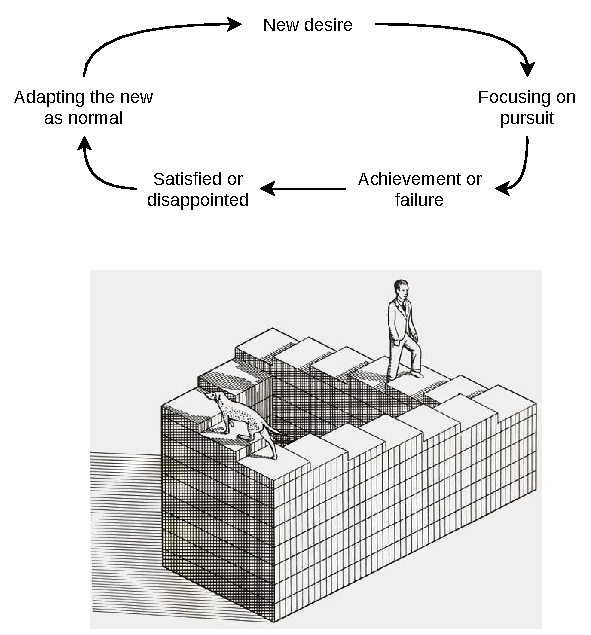
\includegraphics[width=80mm]{hedonic-treadmill-stairs.pdf}

The Hedonic Tredmill is tendency that new achievements are adapted as the normal level,
and the level of happiness returns to the same level as before.
After one desire is satisfied, the conditioned craving seeks a new state.

\bigskip

From the perspective of the person on the Penrose Stairs,
they are getting further and higher.
From our perspective, we see that they return to the same level as before.

\bigskip

Recall the definition of Noble Truth of the Origin of Suffering:
`It is this craving which leads to renewed existence,
 accompanied by delight and lust, seeking delight here and there;
 that is, craving for sensual pleasures, craving for existence,
 craving for extermination.'
(\href{https://suttacentral.net/sn56.11/en/bodhi}{SN 56.11})

\end{figure}

\clearpage

We can find a persuasive logic in it, and our reasoning for being
critical can be completely reasonable! Psychologists say that the most
difficult patients are the ones who intelligently defend and justify
their own bad habits. We can be so clever, there is absolutely no way to
be happy, and we can prove it. Do you remember yourself playing the role
of such a miserable philosopher?

It is not necessarily an immediate relief when our self-reflection
reveals to us the emptiness of what we have been pursuing. Anger,
despair\footnote{The Buddha compares dealing with anger and despair to
  walking along a path close to a deep drop-off.
  (\href{https://suttacentral.net/sn22.84}{SN 22.84}, With Tissa)} and
sadness can be the first reaction, generating thoughts of self-aversion.
We can recognize that these mind states are not reliable, and on top of
it they shut down our intelligence, and who wants that?

\keywords{patient endurance, gratitude, no hurry}

Patient endurance is an underappreciated virtue, but often, all we need
is to remember to wait: the dramatic rain and thunder of turbulent
mental states will run themselves out. When the sense of gratefulness
appears, it is a sign like the rainbow after a storm. It accompanies
wholesome mental states, and we can intelligently see the situation from
more than one angle: this is a good base for generating helpful thoughts
about what to do. Sometimes, the best is to simplify and turn away from
certain habits and values. Other times, our view has changed and we
might wish to keep up what we have been going, but leaving the big hurry
behind, we continue for the sake of living it, not for the sake of some
elevated emotional or mental state in the future.

\begin{quote}
One should not revive the past\\
Nor speculate on what's to come;\\
The past is left behind,\\
The future is unrealized.

\bigskip

\quoteRef{%

\href{https://suttacentral.net/mn131}{MN 131}, One Fine Night

}
\end{quote}

\section{Humour and Irony}

\keywords{opinions, changing perspectives, noticing what is pleasant}

There are morose, dark moods which are like a logic trap of our own
making. The more we think about it, the more entangled we get in them.
Humour and irony are funny because they show the situation from
unexpected, odd angles. If the logical path straight ahead is blocked,
why not try the sideways track where the fox goes? A joke wouldn't be
funny if it was logical and reasonable. Humour and irony, directed
toward ourselves, are good friends when our usual reasonable thoughts
only create more reasonable suffering.

What makes the old and wise men \emph{wise}? Medical studies\footnote{\href{https://www.researchgate.net/publication/258190619_Aging_irony_and_wisdom_On_the_narrative_psychology_of_later_life}{Aging,
  irony, and wisdom, William Randall (researchgate.net)}} investigated
the various attitudes of senior citizens, and found that an inclination
toward self-directed humour and irony (i.e. being able to laugh at
oneself) allows them to face the significant challenges of ageing and
maintain mental balance and a positive outlook on life.

One of their key observations is that humour and irony develops our
ability to see ourselves from multiple viewpoints. We can fill the role
of the accurate historian and the jesting comedian at the same time.
Hence we are able to see events from multiple narrative angles, and not
being caught in a single story, the frame of the narrative we see
ourselves in remains open, moving toward a positive future. The limits
of our being don't necessarily mean the end of the story, and the laughs
are not hard to find: in the absurd corners of life there is always a
joke to tell.

It can be rude to joke about somebody else's bad situation, but who is
going to get upset over your humorous comments about yourself? If you
feel awful, how about an awful joke? It's a trip that is so bad it's
good, and the tickets are free. `I am an animated skeleton in a skin-bag
with clothes on, standing here with a fabulous hair-cut, I can prove the
logic of \emph{my important} opinions.' What's not to laugh at?

We say that in meditation we observe our own mental habits, but
sometimes we practise this with a critical bias, and observe the
\emph{bad mental habits}, while we don't notice the good ones. It is
possible to become so good at ignoring pleasant mind states, that one
genuinely believes happiness only exists for other people. When
something good happens and you feel happy, stop and notice it, `Hey,
this is nice.' This increases our capacity to recognize and experience
it. Who will notice it if you don't?

\section{Expectations}

\keywords{symbol of Buddha statues, changing predictions, relinquishment}

One might look at a Buddha statue and expect oneself to meditate in the
same perfect posture without moving, like the Buddha. But in this case
we missed the real message, which points to inner qualities rather than
external signs. A Buddha statue is not a depiction of the Buddha, the
historical \emph{Siddhattha Gotama} who lived in the 5th century BC. We
don't have a statue of him made during his lifetime. We know from the
\emph{suttas} that he instructed the monks to \emph{not} create statues
or images of him, and focus on the Dhamma, the truths of the mind
instead. The first Buddha statues were made four or five hundred years
after his death, by Greeks in the Gandhara region of Afghanistan. The
statues represent the wisdom and serenity of the awakened mind,
expressed in the human form.

They are beautiful to look at, but nobody is going to become a Buddha
statue, just like you can't become the photo of the perfect meditator,
or the hero in lyric poem. They do offer advice, but the advice can't
orient us when taken rigidly. We should apply the advice by taking our
inner experience and the present situation into account -- this way we
return to the awareness which awakens to the truth and overcomes the
obstacle. The practice of virtue and trust in the examples of skilful
teachers is a strong foundation. We can wish ourselves to be well and
still admit we are feeling awful, when that's how it is.

Expectations are a prediction of the expected value of a result, they
estimate the outcome of our situation. Meanwhile, every factor which
goes into that prediction is undergoing change. We have to allow the
prediction to change, our expectations of our mental experience must
keep changing according to where we are now. Having expectations is not
a problem, but if we attach to a particular outcome which we believe to
be `the real one', this becomes a hindrance. It turns out that if we
invest in future emotional states as the basis of our happiness, the
result is disappointment.

The \emph{ānāpānasati} breathing technique taught by the Buddha has
sixteen steps. The first is knowing whether the breath is long or short,
what might be the last step? We might wonder, `What could be that
exalted mind state, which we will reach?' The instruction leads us to
realize that this is not the correct attitude. The breathing meditation
teaches the contemplation of the body, feelings, and mental states,
followed by contemplating natural truths, of which the last step is:

\begin{quote}
He trains thus: `I shall breathe in contemplating relinquishment'. He
trains thus: `I shall breathe out contemplating relinquishment'.

\bigskip

\quoteRef{%

\href{https://suttacentral.net/mn118}{MN 118}, Mindfulness of Breathing

}
\end{quote}

The practice of the Eightfold Noble Path is not about accumulating, but
about transforming our values through observation and alert
investigation of the experience of changing conditions. At the end we
relinquish them, like putting down a burden and not carrying it any
further. This includes all that we take to be `me and mine': and anyway,
how long can we hold onto anything?

\keywords{real practitioner, Impostor Syndrome}

Reflection and cultivation allows for change, and opens up a wide field
of view where opposites can exist in complex relationships. In a
contrasting approach, the judgmental and comparing mind limits our
scope, it wants to sort things into neat, mutually exclusive abstract
categories. This latter attitude leads to mistrust and harm -- we start
losing faith, not believing ourselves to be `real' practitioners, and
others don't seem to be credible ones either. The result is that we
can't learn from ourselves, and we can't accept anyone to teach us
either. This doubt is blinding and paralysing, it feels like we can't do
anything, when the problem could be that our expectations are too
narrowly focused.

It's not that there are no problems and difficulties. Telling ourselves
that pain is not painful is not a meditation technique taught by the
Buddha. We invent it as a cover story when we think we should be like
mythological ideals. Meditation is not a power to control mental states,
but cultivating awareness, so that they don't control us.

\clearpage

\section{Calibrating}

\keywords{emotions, disappointment, adjusting expectations}

Medical research tells us that a particular emotion is comparable to a
prediction.\footnote{\href{https://www.goodreads.com/book/show/23719305-how-emotions-are-made}{How
  Emotions Are Made: The Secret Life of the Brain by Lisa Feldman
  Barrett}} Our brain evaluates the present based on the past, and
reacts according to whether good or bad can be expected. The brain is
constantly receiving signals from the nervous system, and based on what
it had learnt, it is trying to predict whether the present situation is
going to mean energy input or energy expense for the body. It formulates
the response through hormones, which create the bodily reaction, such as
fear of danger, excitement of immediate reward or euphoric happiness.

We tend to believe that our experience is like the view when we look out
through a window: We stand in front of it, take in the view through our
senses, and have a more-or-less complete picture of `what is out there'.

It turns out that the picture is rather less complete than we think,
when we consider how the senses and the nervous system work. The brain
doesn't have much information to work with, and so it has to guess from
simple signals, hints about what the rich world outside of itself might
be like.

It can't see much: it's sitting in the skull, which is a dark box.
Bodily fluids, chemicals and nerve signals carry messages into this box.
The messages come from other systems in the body, which are themselves
noisy and sometimes conflict each other. From this clutter, the brain
has to create a perception of where we are, guess what is happening to
us, make a prediction of what is likely to happen in the next minute or
so, and produce a response which is hopefully going to help us survive,
or even lead to happiness. It has to do all this, from inside a dark
box, based on a few noisy and limited signals.

What am I then, an animated skeleton, and my head is a dark box? That
explains a lot of confusion. Is it a wonder that my predictions are a
bit off, and need constant adjusting? What I experience as reality is an
ongoing guesswork, changing by the second.

`Happiness equals reality minus expectations' -- a memorable phrase by
Tom Magliozzi. These days, our expectations are so high. We receive
updates from social media apps, we read web articles, and each time they
influence our view of how we are, and how the world is. They show us an
impossibly perfect, impossibly determined, or impossibly outrageous
image of other people. Since we don't meet these people face-to-face, we
don't see the real background of their lives, and this exaggerates our
expectations. It trains the brain again and again to expect these
artificial presentations, like an expectation machine on overdrive. We
don't even notice the distorted self-conditioning, but our
dissatisfaction creates feelings of disappointment and exhaustion.

\keywords{simplicity, impermanence, self-reflection, values}

We \emph{can} calibrate the `expectation machine' through the balancing
effect of conscious reflection and reasoning. `What are the most
essential duties to take care of today? Materially, what do we need for
one day?' When you simplify the answer down to the essentials, it's not
that much. Food, clothes, shelter, medicine, supportive companions and
perhaps something to do toward a worthwhile goal. The average day is not
going to hold to this abstract, pure simplicity, but this is for
recognizing the baseline. If simple is enough, it is not a problem to be
able to do more, or have access to more, contentment remains our
baseline. Ambition is not the problem, but hyping up the expectations
blocks its application.

Expectations are necessary to follow a given direction in the world, but
not understanding them, they become obstructions in the heart. The
expectations and emotions have the nature to arise, then twist,
flip-flop and turn around. Allow them to pass on, like leaves in the
water next to a boat. Bad ones are not that bad, good ones are not that
sure. Knowing their changing nature, we don't take them so seriously and
don't get stuck on them, as a boat shouldn't get stuck on some dry
leaves.

\begin{quote}
Whether it be pleasant or painful\\
Along with the neutral,\\
Either internal or external,\\
Whatever feeling there is:\\
Knowing them, `This is suffering,\\
deceitful and disintegrating,'\\
Coming in contact again and again,\\
seeing their fall,\\
One loses one's passion for them.

\bigskip

\quoteRef{%

\href{https://suttacentral.net/sn36.2}{SN 36.2}, Pleasure

}
\end{quote}

\clearpage

\section{Human Flourishing}

\keywords{meanings of happiness, results, day-by-day practice, death, contentment}

Our modern Western culture often presents happiness as a particular
feeling, or a certain situation in life where we should arrive at. We
pass on our culture by discussion with one another, and our way of
talking about happiness tends to treat it as an outcome, an event in the
future, or a certain state of being. This seems to be a recent trend,
and not necessarily a helpful one.

Traditionally we view the ancient Greeks as one of the most influential
societies in the formation of our Western values, and among others,
Aristotle (384-322 BC) as one who stands out among them. A good
collection of his writings have survived in a form still accessible to
us, and in these he investigates the question of happiness in great
detail.\footnote{\href{https://plato.stanford.edu/entries/aristotle-ethics/}{Aristotle's
  Ethics (plato.stanford.edu)}} It concerned him what happiness is, and
how to live a happy life, but, he saw the experience of happiness not as
a particular outcome or result.

The Greek word he used for `happiness' was \emph{eudaimonia}, translated
as `human flourishing, prosperity.' He saw it manifesting as a
continuously active process which we practice day by day, rather than an
eventual outcome in the future. He describes the practice of happiness
based on moral virtue and a truthful view of one's life from birth,
growing up, old age, and including the tragedy of one's own death.

This direct view of virtue and mortality puts things in order: it gives
us a wide perspective in which happiness has a foundation in wholesome
mental qualities, but we look beyond ourselves to give lasting meaning
to it. Training our expectations in this way, the practice of happiness
is a complete whole every day. We learn to be with the struggle when
that's how it is, applying our best abilities in virtuous ways, and at
the end of each day we can look back with contentment.

If the field of `happiness research' in psychology, Daniel Kahneman and
his team conducted interviews asking people to recall the episodes of
the previous day and later answer questions about them.\footnote{\href{https://www.goodreads.com/book/show/11468377-thinking-fast-and-slow}{Thinking,
  Fast and Slow by Daniel Kahneman}, Day Reconstruction Method} They
confirmed that attention and recurring thoughts are dominant factors in
whether one feels happy or depressed. Even though people were going
through a variety of everyday situations, how they felt was determined
by what they were thinking about at the time.

\keywords{deathbed regrets, life as a unit of time, hierarchy of needs, self-transcendence}

But it surprised them to find that when people spoke about what kind of
day they had, they didn't focus on happiness as a good feeling, but
rather on social experiences, friends and relatives, who did they meet
and what did they do, and on whether they felt satisfied with their life
or not.

All this makes sense when you remember your experience, how much the
perspective, the frame through which we see the world orients us, while
the content of the frame continues to change. The hungry person sees the
world in terms of food, and where to get it. A person in an ambitious
mood focuses on `what I can do' and `how good I am'. A person who is
considering the limited time of the existence of the self is going to
start turning toward values which are self-transcendent, not created by
the self, but timeless qualities apparent here and now.

It was a discovery for me when I heard psychologists discuss a new
addition to Abraham Maslow's hierarchy of needs. Usually pictured as a
pyramid starting with the need for food and water at the bottom, with
self-actualization elevated to the pinnacle. This seemed to be an
ego-centric way of thinking about happiness. The psychologists recently
re-discovered Maslow's late writings,\footnote{\href{https://bigthink.com/neuropsych/maslow-self-transcendence/}{Maslow's
  forgotten pinnacle: Self-transcendence (bigthink.com)}} and found that
toward the end of his life, he felt conflicted about this
value-hierarchy: he was going to die, fundamental parts of his needs
(e.g. survival) were lacking, hence he should be miserable, but instead,
he felt relief and states happiness which he called `peak experiences':

\begin{quote}
`Feelings of limitless horizons opening up to the vision, the feeling of
being simultaneously more powerful and also more helpless than one ever
was before, the feeling of great ecstasy and wonder and awe, the loss of
placing in time and space with, finally, the conviction that something
extremely important and valuable had happened, so that the subject is to
some extent transformed and strengthened even in his daily life by such
experiences.'
\end{quote}

He appended another level to his hierarchy of needs:
\emph{self-transcendence}. Examples are: not holding onto perfection and
one's opinions, giving up the need for certainty and the attachment to
one's past, letting go of the fear of death.

`Self-transcendence' sounds like something for a Buddha, but since we
are suffering from our attachments to one thing or another, it turns out
to be a basic \emph{need} for all of us. Holding onto what we think we
are creates the very limits which we struggle with, wanting to expand
but being held back by grasping an identity. When that identity turns
out to be an empty void, we urgently need help. Think of the day-to-day
struggles, being conflicted over opinions, stressed out about our
abilities, anxious due to unexpected changes, lamenting past tragedies:
we \emph{need} a self-transcendent perspective to get over ourself.

Still, we do keep the score on how our things are going, don't we?
Wholesome conditions are our supports. This is the time and place where
we live, not another: \emph{memento vivere}, remember to live. We know
if our efforts are aligned with our core values or not, even though we
can get distracted with things we didn't mean to spend so much time on.
I remember how it shook me up when I read that some of the most common
deathbed regrets heard by nurses included working too hard and losing
touch with old friends.\footnote{\href{https://bronnieware.com/blog/regrets-of-the-dying/}{Regrets
  of the Dying (bronnieware.com)}} Life is a unit of time with a
beginning and an end, and we should treat it as such.

\keywords{\emph{memento mori}, \emph{memento vivere}, \emph{amor fati}, \emph{saṃvega}, \emph{pasāda}}

If tuning the mind to a comfortable numbness is `tranquillizing
ourselves with the trivial' as mentioned earlier, then recollecting
death (\emph{memento mori}) is a dose of anti-tranquillizer. Since the
time is limited, we remember the urgency to live (\emph{memento vivere})
and do what must be done before it's too late. This motivates us to find
the courage to be true to ourselves and turn toward the situation we are
in (\emph{amor fati}), not waiting for some place and time we imagine in
the future. In the Pali language of the Buddhist \emph{suttas},
\emph{saṃvega} refers to the sense of spiritual urgency, while
\emph{pasāda} expresses the serenity of having confidence in the Path
and its practice.

Reading about deathbed regrets was a timely reminder for me to think
about the urgency I felt about completing projects (which come and go by
the month), and not losing the opportunity of spending quality time with
long-time companions. Reflecting on life as a single unit of time
includes being born, growing and dying. Remembering our mortality this
way puts our values back in line with nature, where we can give
ourselves some space to dwell where we are, and appreciate it before its
over. We seem to understand the fleeting nature of good and bad
feelings, compared to the importance of our golden relationships, even
though we can be caught up complaining about the former and neglecting
the latter.

We can remember that we wish ourself well-being and happiness, and we
wish our family and friends happiness in their life. Consciously
recollecting moral virtues builds mental resilience and self-respect.
Either when we see it in others, such as in teachers and role models, or
in our own experience. It develops gladness and appreciation of what is
good in other people, sharing in their successes. There is wellspring of
happiness in cultivating the face-to-face companionship of friends whom
with we are genuinely glad at each other's successes. We can use humour
to ease up a bad mood, and complete the next step forward.

The present is change itself. We bring that experience into awareness
and contemplate the body, feelings, mind states and natural truths
following the refrain in the \emph{Satipaṭṭhāna Sutta}:

\begin{quote}
\ldots{} He dwells contemplating its nature of arising, or he dwells
contemplating its nature of ceasing, or he dwells contemplating its
nature of both arising and ceasing. \ldots{} And he dwells independent,
not clinging to anything in the world.

\bigskip

\quoteRef{%

\href{https://suttacentral.net/mn10}{MN 10}, Mindfulness Meditation

}
\end{quote}
